\subsection{Sensordaten-Fusion}
\label{headtracking_fusion_subsec}
Die Sensordaten-Fusion beschreibt die Verknüpfung von mehreren Sensoren um Informationen besserer Qualität zu gewinnen.
In diesem Projekt gilt es, die aufbereiteten Daten aus beiden Gyroskopen, Beschleunigungssensor und Magnetometer derart zu fusionieren, dass letztlich die zu ermittelnde \emph{Orientierung} des Kopfes möglichst exakt bestimmt werden kann.
Da die bereits vorgestellten Sensoren jeweils Vor- und Nachteile haben, müssen diese bestmöglich ausgenutzt werden.
In den folgenden Abschnitten werden unterschiedliche Fusionsansätze dargestellt und entsprechend der Aufgabenstellung des Projekts bewertet. 

\subsubsection{Madgwick-Filter}
Die Filterung nach Madgwick \cite{madgwick2010efficient} gilt als neuartiger Ansatz zur Bestimmung der Orientierung basierend auf Gyroskop, Beschleunigungssensor und Magnetometer.
Es wird dabei versucht, die magnetische Distorsion sowie den Bias-Drift des Gyroskopes auszugleichen.
Berechnungsgrundlage ist dafür eine auf Quaternionen basierte Darstellungsform, welche in einem Gradienten-Abstiegsverfahren zum Einsatz kommt.
Vorteile dieses Ansatzes sind seine niedrigen Berechnungskosten, Effektivität bei niedrigen Sampleraten und ein hoher Grad an Parametrisierung, welcher eine Anpassung an die jeweiligen Sensor- und Umgebungscharakteristiken zulässt.

Auch wenn der Madgwick-Filter bereits als fertige \ac{ROS}-Node\footnote{\url{http://wiki.ros.org/imu_filter_madgwick}} vorhanden ist und bessere Ergebnisse als der Kalman-Filter liefern soll, fiel die Entscheidung gegen den Madgwick-Filter aus.
Grund dafür ist, dass der Stand der bestehenden Implementierung nur schwer an den Madgwick-Filter angepasst werden konnte, und dadurch der erzielte Mehrwert so nur schwer nachvollziehbar bzw. verifizierbar gewesen wäre. 

\subsubsection{Kalman-Filter}
Das Kalman-Filter-Verfahren \cite{kalman1960new} ist eine probabilistische Methode der Zustandsschätzung.
Dabei fließen in einem ersten \emph{Prädiktionsschritt} zuvor festgelegte Annahmen inklusive dazugehöriger Fehlerwahrscheinlichkeiten in die Berechnung ein.
Danach wird in einem zweiten Schritt, dem \emph{Innovationsschritt}, eine Beobachtung mit dazugehöriger Messungenauigkeit mit einbezogen.

Um bei einer fehlerbehafteten Beobachtung den Systemzustand zu korrigieren, müssen diese Beobachtungen über mathematische Gleichungen beschreibbar und Fehlerverteilungen für Sensoren bekannt sein.
Diese Informationen sind im vorliegenden Projekt nicht bekannt.
Infolgedessen kann eine Modellierung gemäß dem Kalman-Filter nicht durchgeführt werden. 
Des Weiteren ist unklar, ob durch eine solche Umsetzung tatsächlich Vorteile erzielt werden können, da die Änderung eines plötzlichen Ereignisses (\zB eine Kurvenfahrt) über mehrere Zeitschritte hinweg angepasst wird und somit eine mögliche Latenz hinzugefügt werden könnte.

\subsubsection{Komplementär-Filter}
Nach Brooks und Iyengar \cite{Brooks.1998} hat eine komplementäre Fusion das Ziel, die Genauigkeit von Daten zu verbessern. 
Dabei wirken die Sensoren unabhängig voneinander und liefern unterschiedliche Erkenntnisse und Sichtbereiche, die die Orientierung zu unterschiedlichen Zeiten verbessert.

Die Gyroskope sind wie bereits erwähnt bei einer langen Laufzeit fehleranfällig und erzeugen einen Drift. 
Daher wird im ersten Schritt eine \ac{SLERP}-Interpolation eingesetzt, die bei jedem Zeitschritt die Orientierung der Gyroskope zu $95\%$ und die Orientierung des Beschleunigungssensors zu $5\%$ berücksichtigt.
Hierbei wird das \emph{Roll} und \emph{Pitch} durch Daten des Beschleunigungssensors gestützt und der Gyroskopdrift ausgeglichen.
Der zweite Schritt zielt auf die Verbesserung von \emph{Yaw} ab.
Eine weitere Interpolation verrechnet das vorige Ergebnis mit den aufbereiteten Magnetometerwerten zu $5\%$ pro Zeitschritt.
Formal lässt sich die Gewichtung folgendermaßen beschreiben:
\\
\begin{align}
F_P &= \textbf{\textit{Gyro}}*~0.95~~+~~\textbf{\textit{Acc}}~~*~0.05\\
\notag\\
F_G &= ~F_P~~*~0.95~~+~~\textbf{\textit{Mag}}~*~0.05
\end{align}
\\
Eine Übersicht der Fusionierung mit dem Komplementär-Filter ist Abb.~\ref{fig:fusion_complementary} zu entnehmen.

\begin{figure}[ht]
	\begin{center}
		\scalebox{0.77}{
	\begin{tikzpicture}[%
		>=stealth, % Aussehen der Pfeilspitzen
		->, % Linien als Verbindungslinien
		looseness=.7, % Kr"ummung der Pfeile mit Option ’bent’
		auto, % Position des Ankers f"ur Node Labels
		color=black, % Farbe aller Linien
		%text=red, % Textfarbe in den Matrix-Nodes
		line width=1pt, % Linienst"arke f"ur alle Elemente
		text centered
	]
		\tikzstyle{every node}=[shape=rectangle,draw,fill=white,
		anchor=center] % Stil der Node-Beschriftung der
	% DHA: Die Gewichtung wird bereits durch die Formel vorher klar.
	%\node[rectangle, rotate=-30, draw=orange, text width=2.5cm, outer sep=3pt, minimum size=1.5cm] at (0.6,4.5) {\textbf{$\alpha X+(1-\alpha)Y$}};
	\node[rectangle, font=\bfseries, double=green, text width=2.0cm, outer sep=3pt, minimum size=1.5cm](gyro) at (-7.0,5.5) {Gyro};
	\node[rectangle, font=\bfseries, double=green, text width=2.0cm, outer sep=3pt, minimum size=1.5cm](acc) at (-3.0,5.5) {Acc};
	
	\node[rectangle, font=\small, text width=2.5cm, outer sep=3pt, minimum size=1.5cm](interpol1) at (-3.0,2.5) {Interpolation \\ \textit{(SLERP)}};
	
	\node[rectangle, font=\small, text width=2.5cm, outer sep=3pt, minimum size=1.5cm](interpol2) at (-3.0,-2.5) {Interpolation \\ \textit{(SLERP)}};
	\node[rectangle, font=\bfseries, double=green, text width=2.0cm, outer sep=3pt, minimum size=1.5cm](mag) at (-7.0,-2.5) {Mag};
	
	\node[draw=none] at (-0.5, 0.5)(imageAbove) {\scalebox{0.33}{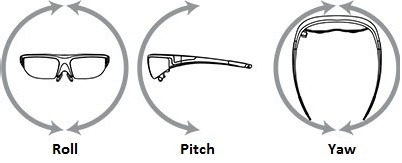
\includegraphics{rpy}}};
	\node[draw=none] at (-1.7, -0.5) {\scalebox{0.02}{
\includegraphics{Yes}}};
	\node[draw=none] at (-0.5, -0.5) {\scalebox{0.02}{
\includegraphics{Yes}}};
	\node[draw=none] at (0.75, -0.5) {\scalebox{0.02}{
\includegraphics{cross}}};
	
	\node[draw=none] at (1.0, -2.5)(imageBelow) {\scalebox{0.33}{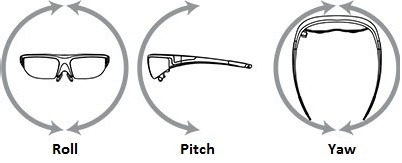
\includegraphics{rpy}}};
	\node[draw=none] at (-0.2, -3.5) {\scalebox{0.02}{
\includegraphics{Yes}}};
	\node[draw=none] at (1., -3.5) {\scalebox{0.02}{
\includegraphics{Yes}}};
	\node[draw=none] at (2.2, -3.5) {\scalebox{0.02}{
\includegraphics{Yes}}};

	\draw[orange, line width=2] (gyro) to[out=-90,in=-180] node[black, above, draw=none, fill=white, font=\small]{$0.95$} (interpol1);
	\draw[orange, line width=2] (acc) -- node[black, above, draw=none, fill=white, font=\small]{$0.05$} (interpol1);
	\draw[orange, line width=2] (interpol1) -- node[black, above, draw=none, fill=white, font=\small]{$0.95$} (interpol2);
	\draw[orange, line width=2] (mag) -- node[black, above, draw=none, fill=white, font=\small]{$0.05$} (interpol2);
	\draw[orange, line width=2] (interpol2) -- (imageBelow);
	
	\end{tikzpicture}}
	\end{center}
   \caption[]{Fusion -- Komplementärfilter}
   \label{fig:fusion_complementary}
\end{figure}

% TR: Voll die gute Abb.!!  :-)
% FG: Nicht der Rede Wert.. ;)
